\begin{figure}[t]
    \begin{minipage}{\columnwidth}
        \begin{center}
            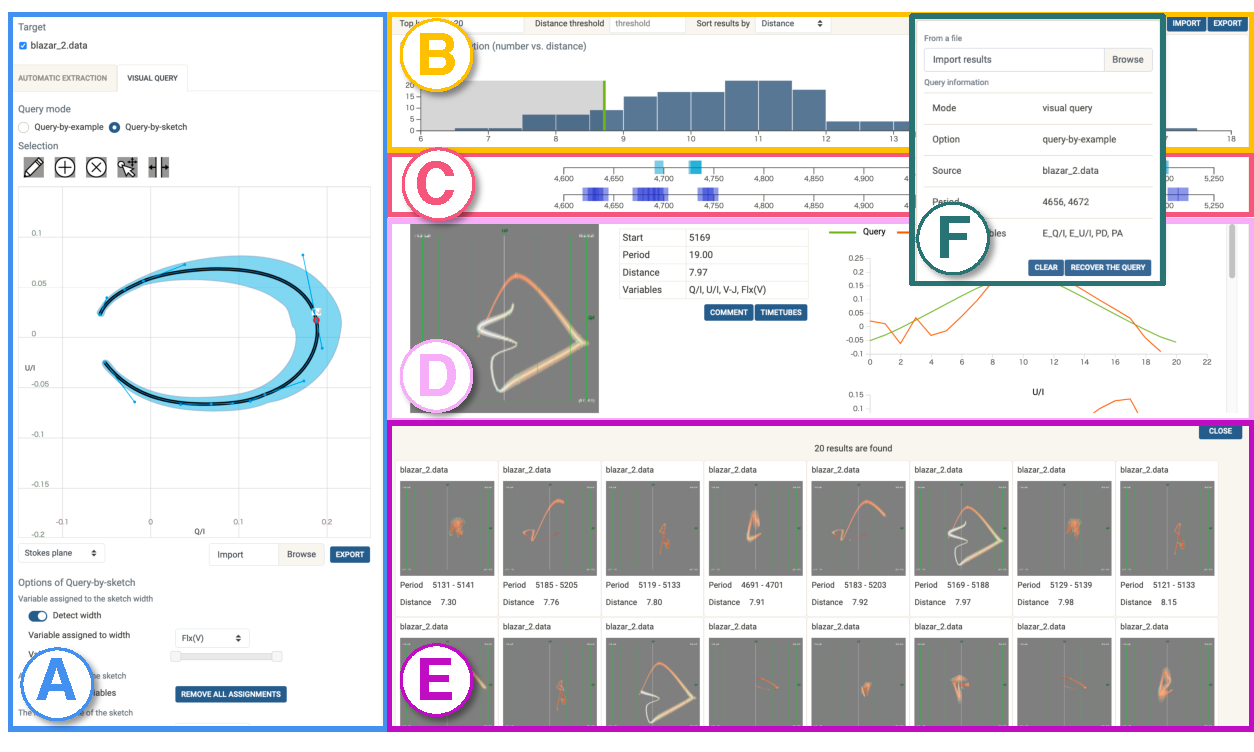
\includegraphics[width=.99\linewidth]{figures/GUI.pdf}
        \end{center}
        \begin{minipage}{\columnwidth}
        \caption{
        The user interface for interactive feature analysis. (A)~Query specification panel; (B)~parameters for ranking, filtering, and displaying extraction results and a histogram for the distribution of distances returned by the similarity search; (C)~timelines overviewing displayed extraction results; (D)~a detailed information panel for a selected result; (E)~a collection of thumbnails for extraction results; and (F)~summary of the imported previous extraction results.}
        \label{fig:UIFeatureExtraction}
        \end{minipage}
    \end{minipage}
\end{figure}
\begin{figure}[t]
    \begin{minipage}{\columnwidth}
        \begin{center}
            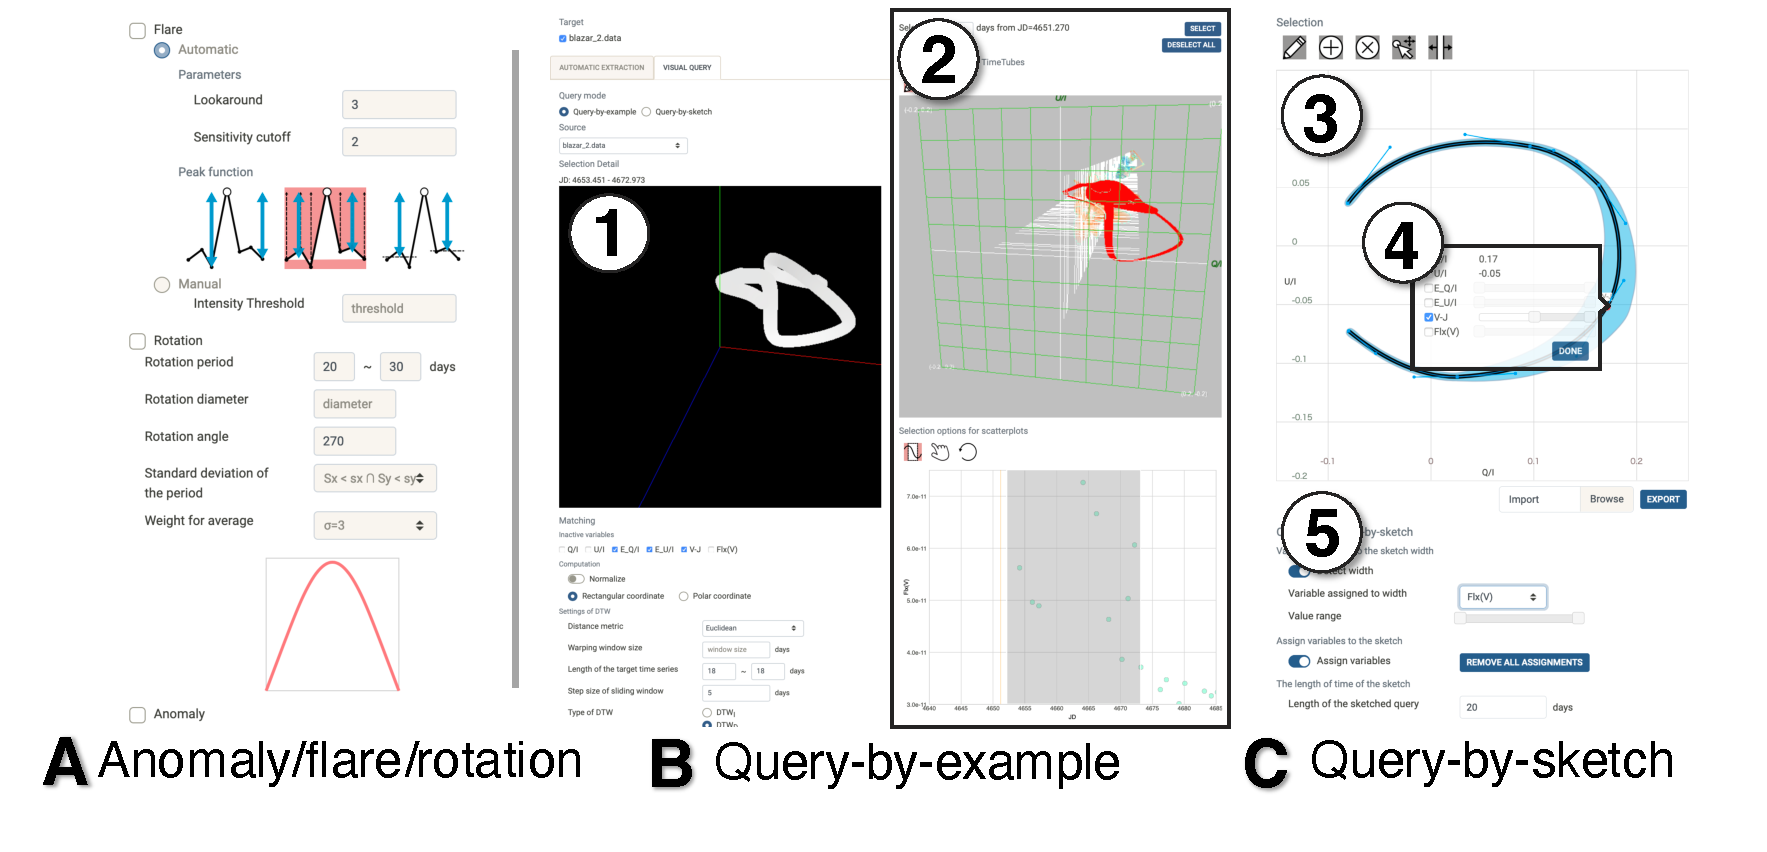
\includegraphics[width=.99\linewidth]{figures/QuerySpecificationPanel.pdf}
        \end{center}
        \begin{minipage}{\columnwidth}
        \caption{Query specification panels for feature and pattern detection methods. (A) Automatic feature extraction; (B) query-by-example, where users can check the selected time interval in a 3D tube view and further fine-tune query parameters (1) after selecting a time interval in the TimeTubes or scatterplots views (2);
         and (C) query-by-sketch, where users draw a SOI (3) and assign filtering constraints at each control point of the hand-drawn sketch (4) or adjust sketch pad settings (5).}
        \label{fig:querySpecificationPanel}
        \end{minipage}
    \end{minipage}
\end{figure}
\begin{figure}[t]
    \centering
    \vspace{3mm}
    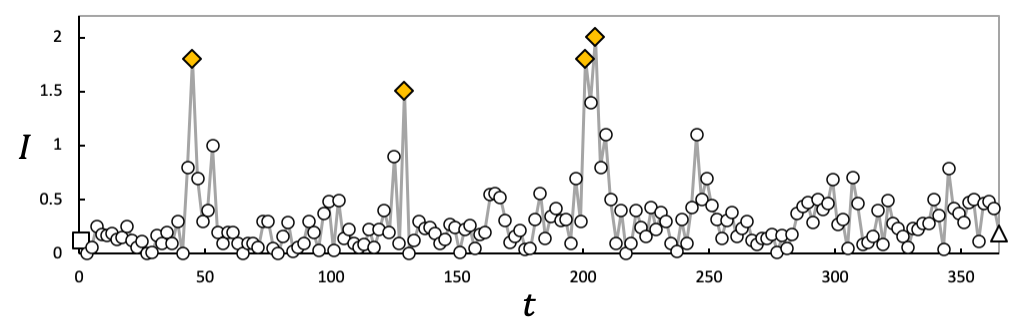
\includegraphics[width=.8\linewidth]{figures/synthesisDataLightCurveLabel_revised.png}\\
    \footnotesize{\sf (a) Light curve plot. The orange diamonds indicate peaks in the data.}\\
    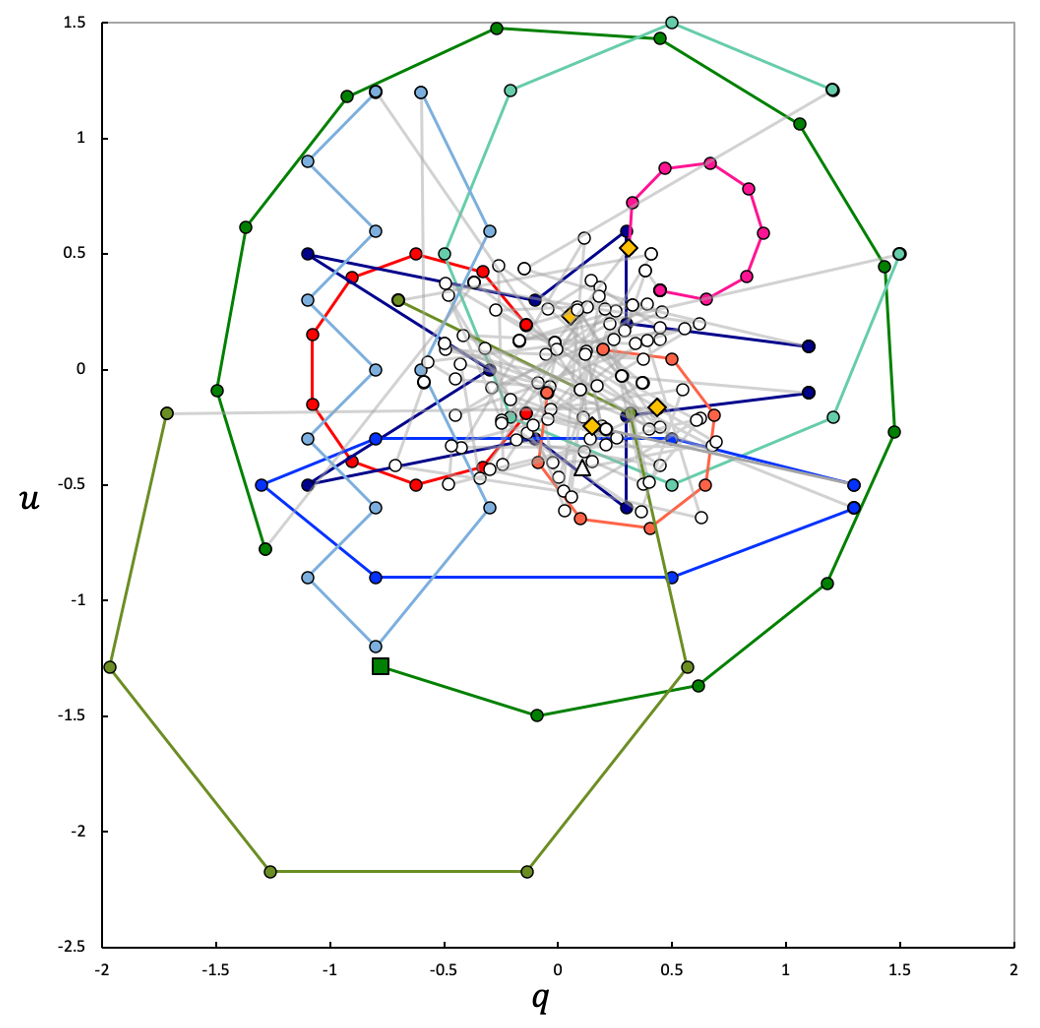
\includegraphics[width=.83\linewidth]{figures/synthesisDataStokesLabel_revised.png}\\
    \footnotesize{\sf (b) Stokes plane plot. The orange diamonds indicate the peaks in (a).}
    \caption{Conventional light curve plot and the Stokes plane for our synthetic dataset. The data has three small circular patterns (red), three large rotations (green), and three narrow/rough-edged patterns (blue) within 365 days. Data starts from the square mark and ends at the triangular mark.}
    \label{fig:synthesisData}
\end{figure}
\section{Automatic Feature Extraction}\label{sec:automaticExtraction}
Astronomers pay careful attention to unusual behaviors of blazars, such as flare and rotation.
As a first step to identify flares and rotations (\textbf{G2}),
we have implemented automatic feature extraction for the discovery and analysis of dynamic time variations (\textbf{T3}).
TimeTubesX automatically extracts three types of features: anomalies (Section~\ref{sec:anomalyDetection}), flares (Section~\ref{sec:flareDetection}), and rotations (Section~\ref{sec:rotationDetection}).
We have significantly improved the detection algorithms for flares and rotations compared with the ones in our previous work~\cite{Sawada2018} 
to identify flares more flexibly and detect rotations more accurately.
Fig.~\ref{fig:querySpecificationPanel} (A) shows the automatic feature extraction panel,
where users can select specific patterns and parameters for automatic feature extraction.
The node (A) in Fig.~\ref{fig:framework} shows example TimeTubes views for an anomaly, flare, and rotation.

\subsection{Anomaly Detection}\label{sec:anomalyDetection}
It is challenging for astronomers to manually identify time variations across multiple variables. 
We define data samples with drastic temporal changes in polarization, intensity, and color as \textit{anomalies}.
Tracking anomalies can result in identifying unusual time variations or presages of well-known behaviors, such as flares or rotations,
because observable blazar behaviors show a tendency to include these drastic variations.

The anomaly degree was defined in our previous work~\cite{Sawada2018} as the product of the change amount in polarization, intensity, and color per day:
\begin{equation*}
\begin{split}
  \int_t^{t + 1}\left|\frac{dPolar(t)}{dt}\right|\cdot\left|\frac{dI(t)}{dt}\right|\cdot\left|\frac{dC(t)}{dt}\right|dt,
  \label{eq:anomaly}
\end{split}
\end{equation*}
where $Polar(t)$ means the position of a data sample on the Stokes plane at time $t$, and $I(t)$ and $C(t)$ stand for intensity and color, respectively. 

\textsf{Experimental results.\ } Applying the anomaly detection to our synthetic data, 
data samples around extreme peaks (the orange diamonds in Fig.~\ref{fig:synthesisData}~(a)) and parts of dynamic rotations (the green plots in (b)) were highly ranked.


\subsection{Flare Detection}\label{sec:flareDetection}
Flares are defined as extreme peaks of brightness (i.e., emitted light intensity). 
Astronomers regard flares as one of the most important observed behaviors of blazars.
However, since there is no specific threshold value of $I$ to define a flare, 
they need to analyze the local temporal profile of $I$ to identify flares.
We have updated the flare detection methods used in our previous work~\cite{Sawada2018}
to detect relatively small local flares as well as globally large flares.
To that end, we utilize peak detection methods for time-series data~\cite{Palshikar2009} to extract flare candidates. 
Flare detection comprises the following two steps:
\begin{enumerate}[nosep, label=\textsl{Step \arabic*}:, ref=\textsl{Step \arabic*}, align=parleft, leftmargin=*]
    \item \textsl{Compute the spikiness score $S$ for each data sample}; \label{algo:flareSpikiness}
    \item \textsl{Filter out data samples with a globally small $S$}. \label{algo:flareFilter}
\end{enumerate}
TimeTubesX uses Equation~\ref{equ:S2} to compute the spikiness score $S$ for \ref{algo:flareSpikiness};
we tested multiple equations for $S$ and empirically found that the following one produces the best results:
\begin{eqnarray}
    S &=& \frac{\frac{\sum_{k=1}^{K}(x_i - x_{i - k})}{K} + \frac{\sum_{k=1}^{K}(x_i - x_{i + k})}{K}}{2}\label{equ:S2},
\end{eqnarray}
where $x_i$ denotes a data sample indexed as $i$ and $K$ denotes the number of neighbors that should be examined.
Equation~\ref{equ:S2} provides the average values of the averages of distances between $x_i$ and $K$ left neighbors and those between $x_i$ and $K$ right neighbors.
\ref{algo:flareFilter} retains only data samples that satisfy $S - \bar{S} > h \times \sigma_{S}$, 
where $\bar{S}$ and $\sigma_{S}$ denote the mean and standard deviation of all computed $S$ values for the dataset, respectively, 
and $h$ is a user-specified sensitivity threshold. 
The original algorithm~\cite{Palshikar2009} merges peaks that are close together into one, 
but we did not adopt this strategy
because astronomers are equally interested in small, individual flares and large, aggregated flares.

\begin{figure}[tb]
    \centering
    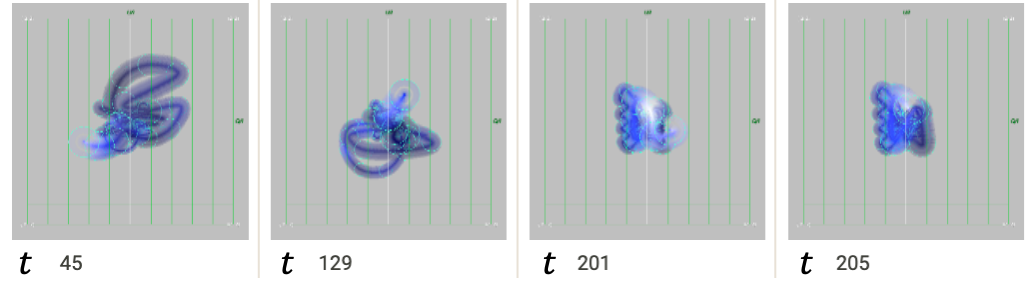
\includegraphics[width=.85\linewidth]{figures/flareDetectiondemodataResults.png}
    \caption{Flare detection results for our synthetic data. The results match the four red data samples in Fig.~\ref{fig:synthesisData}~(a).}
    \label{fig:flareDetection}
\end{figure}
\begin{figure}[tb]
    \centering
    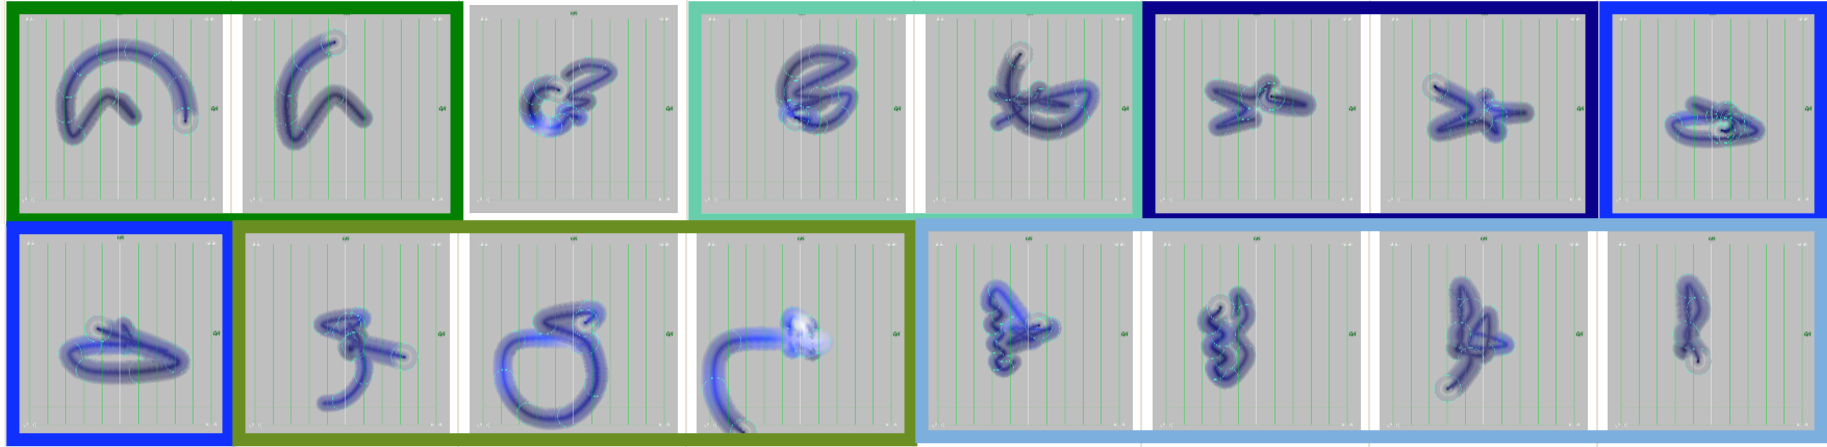
\includegraphics[width=\linewidth]{figures/rotationDetectiondemodataResultsOR.png}\\
    \footnotesize{\sf(a) Previous rotation detection method~\cite{Fujishiro2018}.}\\
    \vspace{5px}
    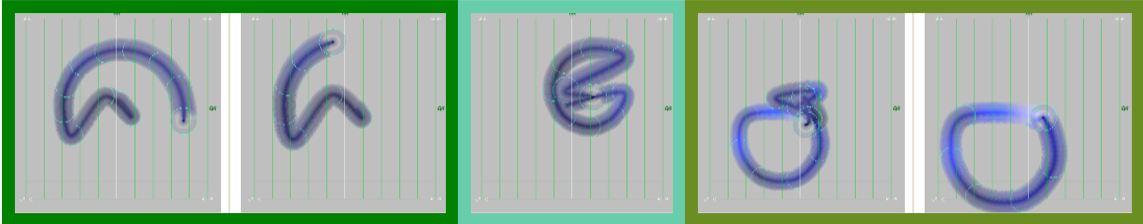
\includegraphics[width=.8\linewidth]{figures/rotationDetectiondemodataResults.png}\\
    \footnotesize{\sf(b) Our improved method.}
    \caption{Rotation detection results for our synthetic dataset in Fig.~\ref{fig:synthesisData}. 
        The outline color corresponds to the color in Fig.~\ref{fig:synthesisData}~(b).
        Our previous method detected narrow/rough-edged patterns and noise (blue), 
        whereas our improved method detected only large rotations (green).}
    \label{fig:rotationResults}
\end{figure}

\textsf{Experimental results.\ } We applied the flare detection method to our synthetic data.
We set $K$ and $h$ to 3 and 1, respectively.
Fig.~\ref{fig:flareDetection} presents the flare detection results.
The four data samples were detected as flares,
which completely coincide with the deliberately generated peaks that are highlighted in orange in Fig.~\ref{fig:synthesisData}~(a).

\subsection{Rotation Detection}\label{sec:rotationDetection}
Polarization rotation is another important observed behavior of blazars. 
Astronomers do not yet agree on whether rotation is an actual feature or just a result of random variations of polarization.
To validate their hypotheses, they scrutinize correlations between polarization and other properties at the time interval.
They typically have been analyzing the time variation of $PA$ to identify rotations~\cite{Ikejiri2011, Uemura2017},
but the rotation center will not be located at the origin of the Stokes plane ($(q, u) = (0, 0)$) when there are multiple polarized components in the sky.
Thus, estimating a rotation only through $PA$ may not allow astronomers to adequately understand its behavior.
Our rotation detection is capable of addressing any rotations regardless of the position of the rotation center.

We use a sliding window approach that allows users to manually define the length of the time interval for the sliding window. Based on feedback from astronomers~\cite{Sasada2012}, we set the default window size to be between three and four weeks.

The computation of the rotation angle is divided into the following seven steps:
\begin{enumerate}[nosep, label=\textsl{Step \arabic*}:, ref=\textsl{Step \arabic*}, align=parleft, leftmargin=*]
    \item \textsl{Compute the weighted means ($\overline{q}, \overline{u}$) of $q$ and $u$ at the time interval};\label{algo:rotationMean}
    \item \textsl{Compute the standard deviations ($\sigma_{q}, \sigma_{u}$) of $q$ and $u$ at the time interval}; \label{algo:rotationStd}
    \item \textsl{Convert the rectangular coordinates ($q-u$ domain) to polar coordinates ($r - \theta$ domain) with its origin shifted to $(\overline{q}, \overline{u})$}; \label{algo:rotationPolar}
    \item \textsl{Filter out time intervals whose $\sigma_{q}$ or $\sigma_{u}$ is smaller than the standard deviations of the entire dataset}; \label{algo:rotationFilter}
    \item \textsl{Compute the difference ($\theta_{\rm diff}$) of the $\theta$'s of two consecutive data samples}; \label{algo:rotationDiff}
    \item \textsl{Sum $\theta_{\rm diff}$'s to yield $\theta_{\rm sum}$}; \label{algo:rotationSum}
    \item \textsl{Check whether $\theta_{\rm sum}$ is larger than the user-specified threshold for the total rotation angle}. \label{algo:rotationThreshold}
\end{enumerate}
We regard $\overline{q}$ and $\overline{u}$ as a rotation center. 
To avoid misleading effects of outliers and unexpected values at the edges of a time interval,
smaller weights are assigned to both ends of the time interval according to a Gaussian distribution at \ref{algo:rotationMean}.
Note that users are allowed to adjust these weight ratios.
To avoid misclassifying time intervals with large $q$ or $u$ variance and unlike rotations as rotation candidates,
we have improved upon our previous rotation detection method~\cite{Sawada2018} on the basis of feedback from two astronomers at Hiroshima University~\cite{Huang2019}.
To detect only large rotations, 
our new method is able to filter out time intervals in which \textbf{either} $\sigma_{q}$ \textbf{or} $ \sigma_{u}$ is smaller than the standard deviation of the entire dataset. 
Note that this and other provided filtering constraints also allow for discovery of small or narrow rotations, such as the red and blue patterns in Fig.~\ref{fig:synthesisData}~(b).
At \ref{algo:rotationDiff}, we cannot compute $\theta_{\rm diff}$ simply by subtracting the $\theta$'s of consecutive observations 
due to the range constraint on $\theta_{\rm diff}$ (i.e., $\theta_{\rm diff} \in [0, 2\pi]$). 
For example, when two successive data samples are located in the first and fourth quadrant of the Stokes plane, 
we need to consider whether to take the clockwise or counterclockwise direction as $\theta_{\rm diff}$. 
We determine the rotation direction 
by checking increasing/decreasing tendency in $\theta$'s with exponential smoothing~\cite{Brown1956}.
It forecasts the next value according to past observations by assigning larger weights to more recent observations.
In this way, it addresses the uncertainty about the rotation direction and make results more feasible (\textbf{T1}).
We estimate the variation trend of $\theta$ and
then define the angle in the predicted rotation direction as $\theta_{\rm diff}$.
Users can set an arbitrary angle as a threshold parameter at \ref{algo:rotationThreshold}.

\textsf{Experimental results.\ } To compare our novel algorithm with the previous rotation detection algorithm~\cite{Sawada2018}, we applied both to our synthetic data.
As the results in Fig.~\ref{fig:rotationResults}~(a) show, 
the previous algorithm detected not only large rotations (green patterns in Fig.~\ref{fig:synthesisData}~(b)) but also narrow or rough-edged patterns (blue).
The improved algorithm more accurately detected only time intervals in which the polarization values dynamically rotate (green), as shown in Fig.~\ref{fig:rotationResults}~(b).
\section{Dynamic Visual Querying}\label{sec:visualQuery}
To facilitate astronomers' discovery of time intervals similar to a ROI/SOI (\textbf{G3}) or those validating specific hypotheses (\textbf{G4}), 
TimeTubesX provides two different user-initiative visual query interfaces: query-by-example (QBE) and query-by-sketch (QBS).
Both are designed to help users identify similar patterns of interest (\textbf{T4}), and our matching algorithm allows for a fuzzy search (\textbf{T5}).

\subsection{Query-by-Example}\label{sec:QBE}
While the TimeTubes view helps users analyze time variations,
it remains challenging for users to build queries for multi-dimensional, time-dependent data.
Our QBE interface allows users to specify a notable behavior as a ROI with simple interactions through the TimeTubes or scatterplots views.
Users can pick a part of time-series data as an input for a query as well as flexibly select specific variables that should be queried about to reflect their intentions. 
This allows users to easily and intuitively search long-term datasets for interesting patterns with minimal required user inputs.

Fig.~\ref{fig:querySpecificationPanel} (B) shows our QBE interface.
To facilitate visual verification by users, a time interval selected through the TimeTubes or scatterplots views in (2, red highlight) is automatically extracted and displayed in the query panel (1).
After selecting the initial time interval, users can then fine-tune and adjust their query by selecting the variables that should be queried about. 
This is crucial for effective support of queries on multi-dimensional data.
Based on the selected variables, 
our system interactively updates the appearance of the 3D tube for the selected time interval in (1), visually encoding only currently selected variables.
For example, when users remove the variable $C$ from the query, the tube loses color variation and becomes a gray tube, as shown in (1).
After defining the query, users can adjust the main parameters (e.g., normalization and polar coordinates options) for our matching algorithm (see Section~\ref{sec:matchingAlgorithm}). 

\textsf{Experimental results.\ } We verified the effectiveness of our QBE method using our synthetic data.
The red circular patterns in Fig.~\ref{fig:synthesisData}~(b) have a similar shape but different time lengths, scales, or locations in the Stokes plane.
We used the leftmost red time interval in (b) as an input query, as shown in Fig.~\ref{fig:QBEDemodata}~(a).
We selected $q$ and $u$ as active variables and used the normalization and polar coordinates options to detect time intervals with different scales or different positions.
The length of the target time interval was set to 5 to 20 days.
We used $\rm{DTW}_{\rm D}$ as a distance function.
Note that we detail the options and parameters related to the matching process in Section~\ref{sec:matchingAlgorithm}.
Fig.~\ref{fig:QBEDemodata}~(b) shows the top three results of our QBE in (a).
The color of the rectangles corresponds to those used in Fig.~\ref{fig:synthesisData}~(b).
We were able to detect all time intervals with a similar shape in our synthetic dataset.
Note that the time interval specified for the query itself is omitted from the results.

\begin{figure}[tb]
    \centering
    \begin{minipage}{0.24\linewidth}
        \centering
        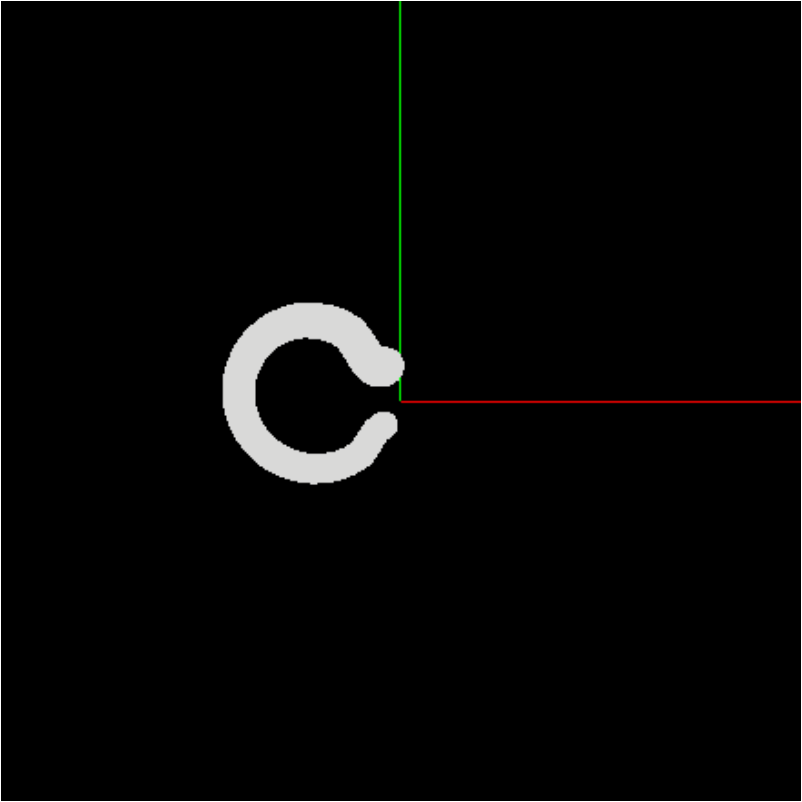
\includegraphics[width=.99\linewidth]{figures/QBE.png}
        \footnotesize{\sf (a)~Query.}
    \end{minipage}
    \begin{minipage}{0.75\linewidth}
        \centering
        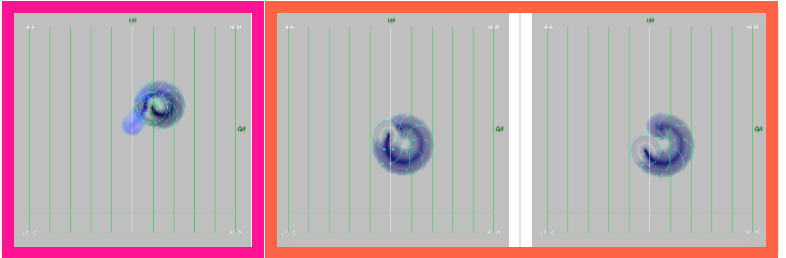
\includegraphics[width=.99\linewidth]{figures/QBEdemodataResults_revised.png}
        \footnotesize{\sf(b)~Results for the query in (a).}
    \end{minipage}
    \caption{QBE for our synthetic dataset in Fig.~\ref{fig:synthesisData}. 
        We chose the time interval with a small circular pattern (the leftmost red pattern in Fig.~\ref{fig:synthesisData}~(b)) for a query in (a). 
        Our method precisely extracted other time intervals with small circular patterns (the two red patterns from the right in Fig.~\ref{fig:synthesisData}~(b)).
        The outline color corresponds to the color in Fig.~\ref{fig:synthesisData}~(b).}
    \label{fig:QBEDemodata}
\end{figure}
\subsection{Query-by-Sketch}\label{sec:QBS}
TimeTubesX also allows users to query their data by manually drawing time variation patterns onto a 2D sketch interface.
Our QBS interface provides an intuitive and accessible way for users to specify patterns for multi-dimensional, semi-structured, time-dependent blazar datasets and validate their high-level hypotheses.
Rouxel et al.~\cite{Rouxel2014} state that an input trajectory by analog gestures is characterized by three dimensions: space, time, and force.
To realize intuitive interactions, 
we use space to determine the $x$ and $y$ positions of the stroke
and use either drawing speed or drawing pressure to define the stroke width 
so that users can describe time variations of multiple dimensions simultaneously.
Using the drawing speed option, the longer a cursor stays on a single point, the wider the curve at the point becomes.
To take into account other variables that are not described in sketching gestures, 
our QBS interface allows users to assign filtering constraints for each variable.
Thus, a sketch-based query for multi-dimensional, semi-structured, time-dependent data can be built with a single gesture
without sketching time variation patterns several times.

Fig.~\ref{fig:querySpecificationPanel} (C) shows the QBS query specification panel.
First, users define which variables are assigned to the $x$ and $y$ axes of the sketch pad and the stroke width (see panel (5)).
Second, they sketch a time variation pattern on a 2D sketch pad UI (3),
where the stroke is shown in black and its width is shown in blue.
Afterward, our system automatically beautifies the input stroke by fitting it to a cubic Bezier curve with as few segments as possible by using the \texttt{\small simplify} method in Paper.js~\cite{paper_framework}.
After their initial drawing, users can further adjust the sketch
by adding, removing, or moving control points or by changing the stroke width.
Users are also allowed to assign filtering constraints to each of the control points on the stroke, as shown in part (4).
They can define value ranges for each variable at the control point, which the algorithm will subsequently use when evaluating the query.

\begin{figure}[tb]
    \centering
    \begin{minipage}{0.49\linewidth}
        \centering
        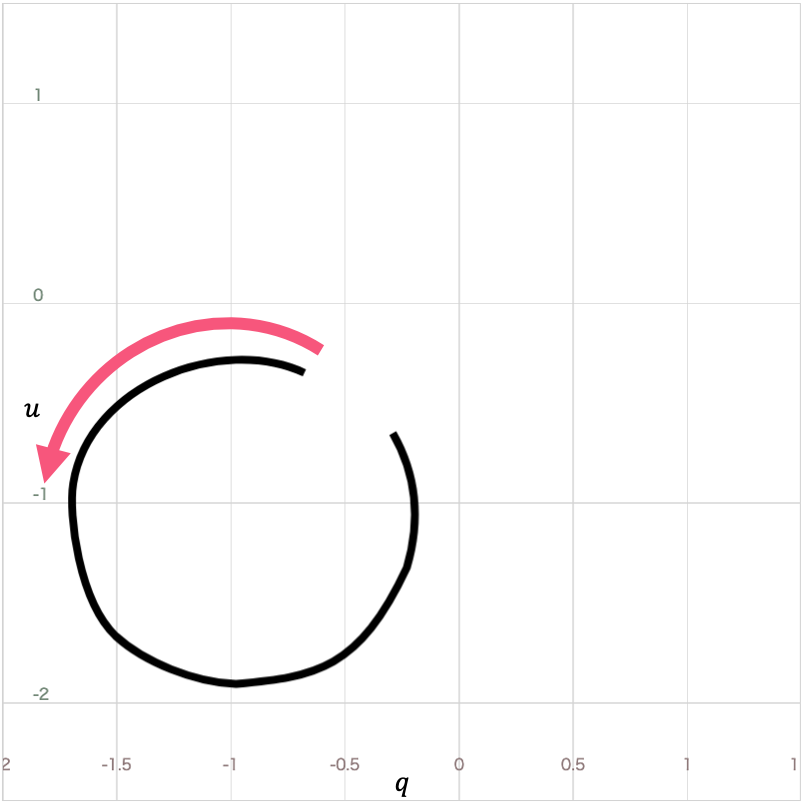
\includegraphics[width=.9\linewidth]{figures/QBSSketchwithoutWidth.png}
    \end{minipage}
    \begin{minipage}{0.49\linewidth}
        \centering
        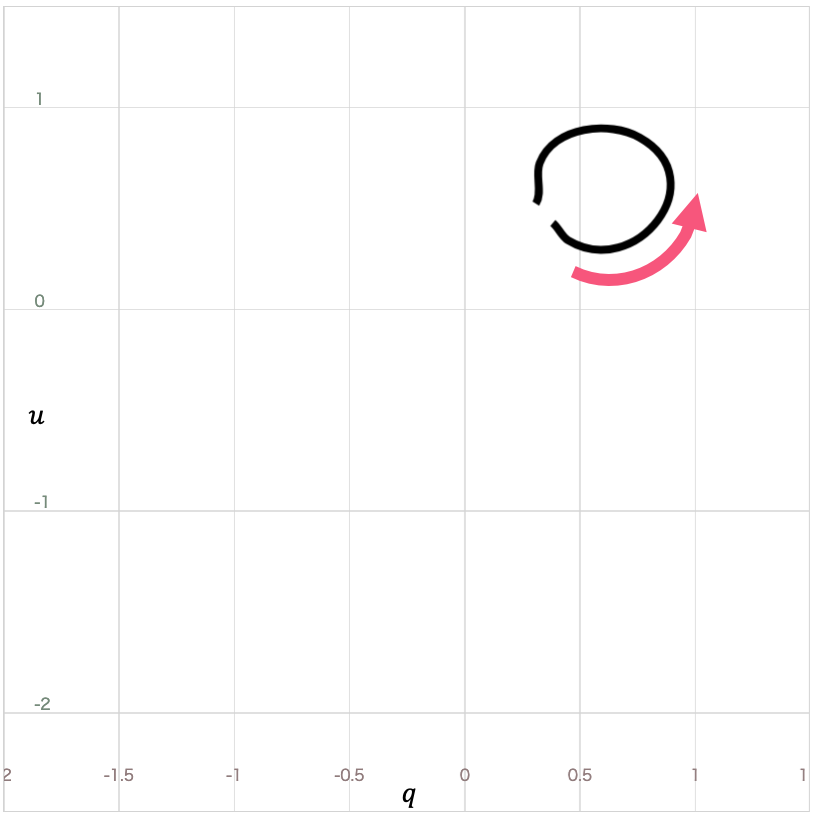
\includegraphics[width=.9\linewidth]{figures/QBSResultQuerywithoutWidth.png}
    \end{minipage}
    \begin{minipage}{0.49\linewidth}
        \centering
        \footnotesize{\sf (a)~A hand-drawn sketch query for a small circular pattern.}
    \end{minipage}
    \begin{minipage}{0.49\linewidth}
        \centering
        \footnotesize{\sf (b)~A sketch based on the upper left result in (c). 
        }
    \end{minipage}
    \begin{minipage}{0.49\linewidth}
        \centering
        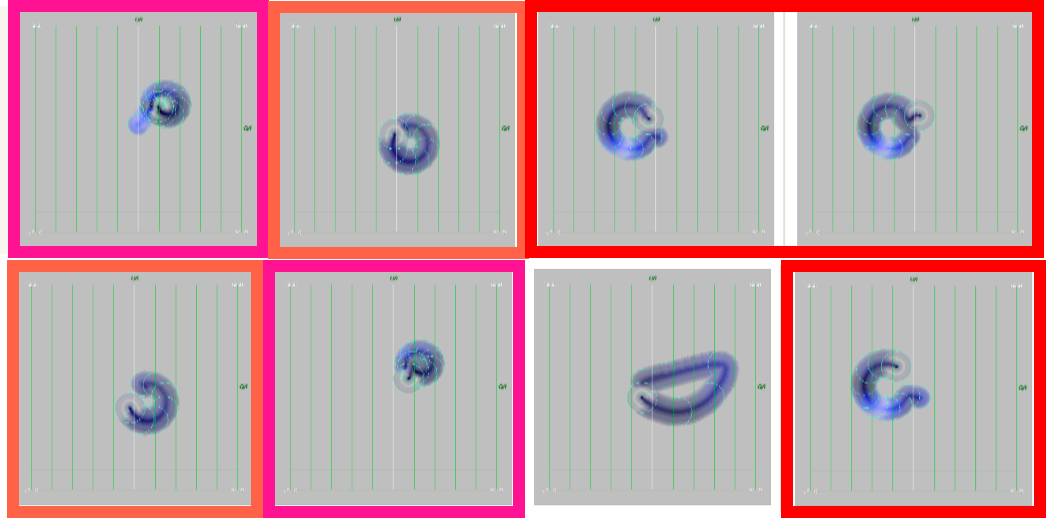
\includegraphics[width=.99\linewidth]{figures/QBSResultsHanddrawn_revised.png}\\
        \footnotesize{\sf (c)~Results for the query in (a).}
    \end{minipage}
    \begin{minipage}{0.49\linewidth}
        \centering
        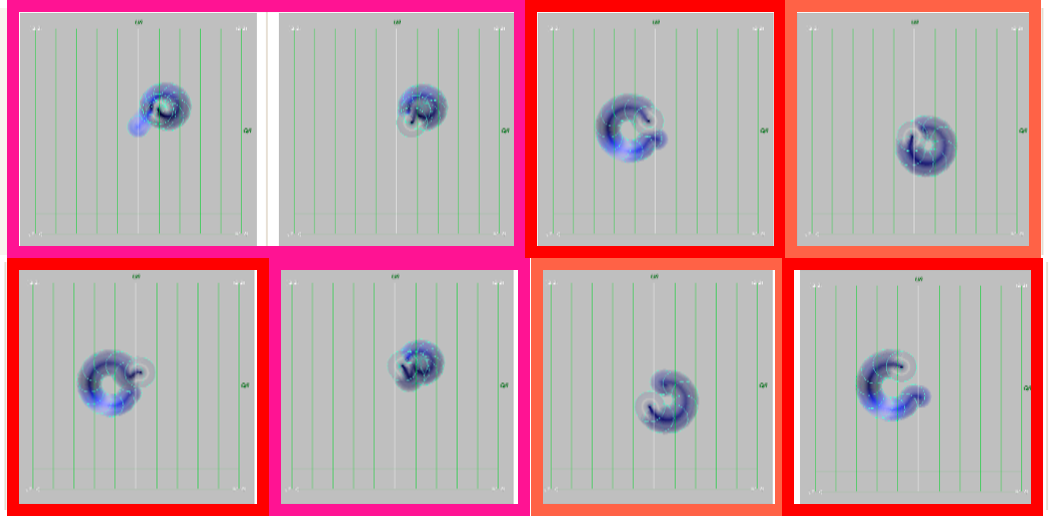
\includegraphics[width=.99\linewidth]{figures/QBSResultsResultQuery_revised.png}\\
        \footnotesize{\sf (d)~Results for the query in (b).}
    \end{minipage}
    \caption{QBS results for our synthetic dataset in Fig.~\ref{fig:synthesisData}.
        On the basis of a hand-drawn sketch in (a), an unexpected result is highly ranked (white outline) in (c). 
        With a sketch based on actual data values (b), no unexpected results appear, as illustrated in (d).
        }
    \label{fig:QBSDemodata}
\end{figure}
\textsf{Experimental results.\ } We evaluated the effectiveness of our QBS method using our synthetic data.
First, we sketched a pattern shown in Fig.~\ref{fig:QBSDemodata}~(a) to extract time intervals with small circular patterns.
The sketch pad plane corresponds to the Stokes plane, and for simplicity, the stroke width is not used.
To detect time intervals with a similar shape but different positions or scales, we used the normalization and polar coordinates options.
Fig.~\ref{fig:QBSDemodata}~(c) shows the top eight results for our QBS in (a).
The outline color of each thumbnails matches the color of the corresponding pattern in Fig.~\ref{fig:synthesisData}~(b).
All three time intervals highlighted in red in Fig.~\ref{fig:synthesisData}~(b) were precisely extracted.
However, an unexpected result (i.e., the thumbnail with white outline in Fig.~\ref{fig:synthesisData}~(c)) was highly ranked as a candidate similar to the input sketch due to the ambiguities of the hand-drawn sketch.
We address this problem by incorporating fact-guided querying (see Section~\ref{sec:factDrivenQuerying}). 

\subsection{Query Matching Algorithm}\label{sec:matchingAlgorithm}
There are many different methods for computing the distance between two time series, such as Euclidean distance, uniform scaling, and dynamic time warping (DTW)~\cite{Berndt1994}.
TimeTubesX uses DTW
because it aligns two time series elastically and thus supports the comparison of time series with different lengths.
Additionally, it can compute the distance between two time series that are similar but locally out of phase.
%more intuitively even if they are out of phase in the time direction. 
According to Eichmann and Zgraggen~\cite{Eichmann2015}, the DTW similarity measurement seems to most closely match human perception.
There are multiple solutions for dealing with multi-dimensional data in DTW. 
TimeTubesX implements two options, ${\rm DTW}_{\rm I}$ (independent) and ${\rm DTW}_{\rm D}$ (dependent), both of which are based on the work of Shokoohi-Yekta et al.~\cite{Shokoohi-Yekta2015}.

${\rm DTW}_{\rm I}$ computes the distance between two time series for each dimension of the data separately. 
In the final step, it adds up all the individual distances to produce the final distance measure.
Consequently, this approach focuses more on the similarity of each dimension and less on correlations between different dimensions.
${\rm DTW}_{\rm D}$, on the other hand, computes the distance between two data samples directly over all dimensions (i.e., as Euclidean distance in $n$-dimensional space).
Therefore, this method focuses more on correlations among the different dimensions of a time series and less on the similarities of individual dimensions. 
By default, our system uses ${\rm DTW}_{\rm D}$ because correlations among variables are important for blazar behavior analysis.
Readers are recommended to consult \cite[Fig. 1]{Shokoohi-Yekta2015} for comprehensive illustrations of ${\rm DTW}_{\rm I}$ and ${\rm DTW}_{\rm D}$.
We use a sliding window approach in our matching algorithm.
Users can set the window size and the step size of the sliding window and also set a constraint on the largest allowed temporal shift (i.e., warping window size)
in the process of finding the best alignment between the query and time series.
Users can specify these parameters at the bottom of the query specification panel in Fig.~\ref{fig:UIFeatureExtraction}~(A).
Note that multiple time intervals with different lengths but that include the same data samples can be presented in the extraction results (see Fig.~\ref{fig:QBEDemodata} and Fig.~\ref{fig:QBSDemodata}~(c) and (d)).
The timelines in Fig.~\ref{fig:UIFeatureExtraction}~(C) help users recognize such time intervals. 

Normalization and polar coordinates options enable a fuzzy pattern search.
The normalization option instructs the system to normalize a query and time intervals into the range of $[0, 1]$.
Subsequently, the pattern search places great significance on the shape of the time variations, whereas the actual value ranges will be ignored.
With the polar coordinates option, 
$q(t)$ and $u(t)$ are converted into polar coordinates ($r-\theta$ domain) before computing similarities.
Subsequently, the pattern search with the normalization and polar coordinates options will also be able to extract patterns rotating around the origin of the Stoke plane.

\subsection{Fact-Guided Querying}\label{sec:factDrivenQuerying}
To support quick and iterative query refinement, TimeTubesX allows users to re-utilize individual extraction results as an input for follow-up queries, a process we have termed \emph{fact-guided querying}.
By iteratively updating a query, users can, in a step-by-step manner, identify more observable time intervals that reflect their intentions.
Therefore, fact-guided querying contributes immensely to drilling down into data as a part of the visual exploration framework of TimeTubesX in Fig.~\ref{fig:framework}.
In QBE, users can switch variables used in the matching process and modify the time range of the query, while in QBS, users can adjust the scale, shape, and axis of the input query or add further filtering constraints.
Thus, fact-guided querying helps users perform further pattern searches based on a time interval of interest found in the previous process or create a sketch-based query from references to actual data measurements instead of from a blank sketch pad.

Our system allows users to build a fact-guided query with simple interactions by, for example, dragging an extraction result either into the QBE interface (part (2) in Fig.~\ref{fig:querySpecificationPanel}~(B)) or into the sketch pad of the QBS interface (part (3) in Fig.~\ref{fig:querySpecificationPanel}~(C)).

\textsf{Experimental results.\ } We confirmed the usefulness of the fact-guided querying approach with our synthetic data.
As discussed in Section~\ref{sec:QBS}, 
hand-drawn sketch queries, such as Fig.~\ref{fig:QBSDemodata}~(a), work well for finding time intervals with a specific feature,
but ambiguities of hand-drawn sketches may sometimes lead to unexpected results, as shown in (c).
If the extraction results for the query in (a) sufficiently represent users' intentions, one of the results can be used as an input to refine the results of the next visual query.
We chose the top left result of Fig.~\ref{fig:QBSDemodata}~(c) and used it as an input for our QBS method, as shown in (b). 
The sketch pad plane in (b) coincides with the Stokes plane.
Thereafter, we ran QBS using the same parameter settings as the example in Section~\ref{sec:QBS}.
As shown in the top eight extraction results in (d),  
this refined query in (b) no longer produces any high-ranking outliers or unexpected results.
\section{Visual Exploration of Query Results}\label{sec:otherFunctions}
In addition to the feature and pattern detection methods described in Sections~\ref{sec:automaticExtraction} and \ref{sec:visualQuery}, TimeTubesX includes powerful visual comparison and annotation features for further analysis of blazar data.

\subsection{Visual Comparison of Query Results}
An essential feature for analysis of blazar datasets is the user's ability to compare query results---not just within a single query but also to previous query results. 
For example, when users find that a specific feature frequently appears in a certain time period,
they might want to investigate whether any other features also frequently appear in the same time period.
Therefore, TimeTubesX can juxtapose the results of different queries
by loading query results that were previously saved as a JSON file.
When importing a file, the stored results are mapped to a new timeline that is arranged as a juxtaposed view below the original timeline.
Hovering over marks on the timeline allows users to see detailed information about specific results.
Additionally, users can re-use or review the settings of the previous query, such as the selected time period or the variables assigned to the sketch pad (see Fig.~\ref{fig:UIFeatureExtraction}~(F)).

\subsection{Annotations of Queries and Query Results}
To enable efficient collaboration between astronomers and to facilitate keeping track of analyses between different sessions, TimeTubesX supports detailed annotations for query results.
Users can access any annotations even after exiting and restarting the application because annotations are stored in the local storage of the web browser. 
To share annotations with other users, annotations can be exported as a single JSON file. 
The system stores the annotation's timestamp, username, comment, and dataset, as well as detailed information about the query and query results.
Users can see all of their annotations in a table view or a single annotation by clicking on a marker with the selected label color in the TimeTubes and scatterplots views.
They can also re-use any query saved in an annotation by simply clicking on it. 

Annotations help users highlight interesting extraction results.
Annotating time intervals of interest not only triggers deeper inspection of a specific period 
but also possibly facilitates the discovery of new features such as periodic patterns.


